\chapter{Моделирование оптической системы}

В качестве источника излучения был выбран ИК лазерный диод FPL1055T с длиной волны излучения 1550 нм, мощностью излучения в импульсном режиме 300 мВт, поперечной расходимостью 28${}^\circ$ и боковой расходимостью 15${}^\circ$~\cite{LDThorlabs}. Выбранный фотодиод \--- FDGA05 с пиковой длиной волны 1550 нм (регистрируемый диапазон длин волн 800\--1700 нм), отзывчивостью 0.95 А/Вт, площадью активной области 0.196 мм${}^2$ и материалом сенсора InGaAs~\cite{PDThorlabs}.

Для моделирования оптической системы использовался пакет Zemax OpticStudio 21.1.2. Рассмотрим задание параметров компонентов системы (рисунки \ref{fig:no_lens_zemax_1}):

\begin{figure}[!h]
    \centering
    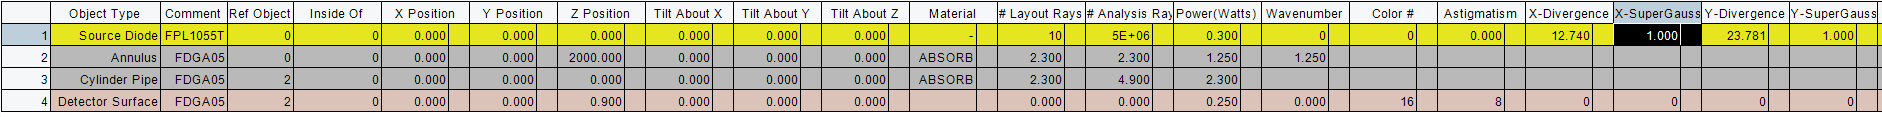
\includegraphics[width=\textwidth]{inc/img/no_lens_1.png}
    \caption{Задание параметров оптической системы в Zemax}
    \label{fig:no_lens_zemax_1}
\end{figure}

Первые 11 колонок (до колонки <<\# Layout Rays>>) универсальны для всех объектов в Zemax: тип объекта, комментарий, референтный объект, нахождение внутри другого объекта, X, Y и Z координаты, наклон вокруг осей X, Y и Z, материал объекта (где применимо). Далее идут специфические для объекта параметры:

Для диода: количество лучей для рендеринга и для расчётов (выбираются произвольно), мощность источника (выбрана в соответствии с~\cite{LDThorlabs}), номер длины волны (задаётся список используемых длин волн, задана только одна \--- 1550 нм, поэтому в ячейке стоит ноль \--- выбор любой длины волны из списка), цвет лучей на рендере, астигматизм (расстояние, на которое смещено распределение излучения в плоскости XZ), расходимость $\alpha_x$ для направления OX, супер-гауссов коэффициент $G_x$ в направлении OX, расходимость $\alpha_y$ и супер-гауссов коэффициент $G_y$ для направления OY. 

Супер-гауссов коэффициент показывает отличие профиля интенсивности данного пучка от профиля интенсивности Гауссова пучка \--- чем он больше, тем ближе профиль интенсивности излучения к прямоугольному профилю~\cite{Paschotta2008}. Для обоих направлений был выбран супер-гауссов коэффициент $G_{x,y} = 1$ (Гауссово распределение интенсивности). Следуя документации Zemax, можно рассчитать $\alpha_{x,y}$ следующим образом: 

\begin{equation*}
    \alpha_{x, y}=\frac{\theta_{\mathrm{fwhm}}}{\sqrt{2 \ln (2)}},
\end{equation*}

где $\theta_{\mathrm{fwhm}}$ \--- угол расходимости из~\cite{LDThorlabs}.

Два следующих объекта формируют корпус фотодиода: круг с отверстием и трубка. Для круга с отверстием задаются радиусы отверстия и самого круга по большой и малой полуосям. Их значения соответствуют размерам реального лазерного диода~\cite{PDThorlabs}. Его положение задаётся относительно лазерного диода.Для трубки задаются радиусы начала и конца, длина. Радиусы равны и взяты из документации к фотодиоду, длина взята произвольной, положение задаётся относительно круга с отверстием.

Для фотодиода заданы размеры апертуры (взяты из документации), количество угловых и радиальных зон оставлены по умолчанию и необходимы для расчётов в симуляции. Положение фотодиода задаётся относительно круга с отверстием и соответствует положению фотодиода в корпусе.

% \begin{figure}[h]
%     \begin{subfigure}{0.5\textwidth}
%         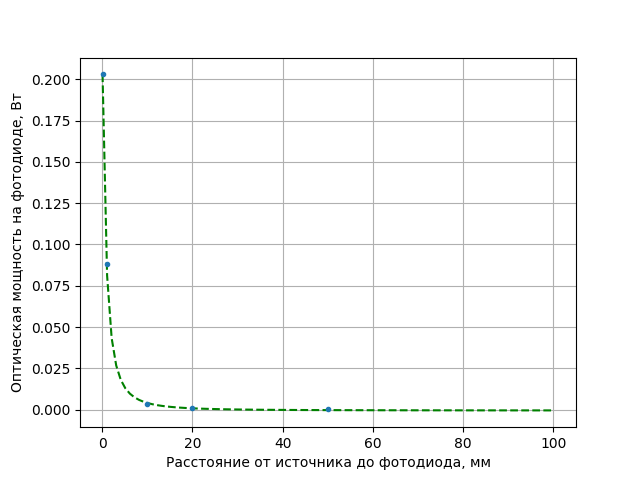
\includegraphics[width=0.9\linewidth]{inc/img/distance.png} 
%         \caption{Caption1}
%         \label{fig:subim1}
%     \end{subfigure}
%     \begin{subfigure}{0.5\textwidth}
%         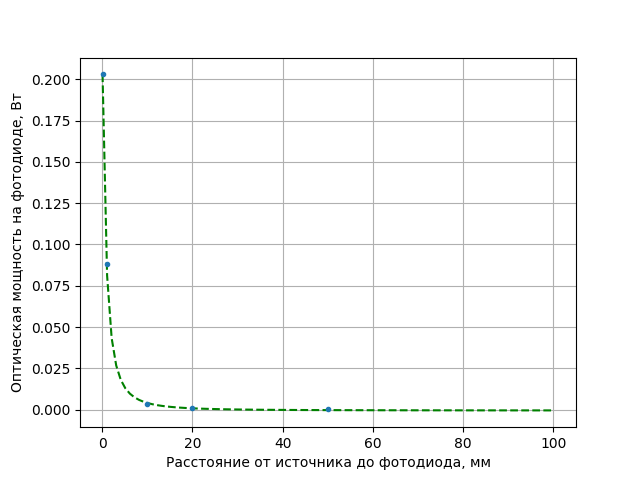
\includegraphics[width=0.9\linewidth]{inc/img/distance.png}
%         \caption{Caption 2}
%         \label{fig:subim2}
%     \end{subfigure}

%     \caption{Caption for this figure with two images}
%     \label{fig:image2}
% \end{figure}

% Что к чему подключали, что измеряли, что измерили
% distance [ 6.14948683e-01  1.63946010e+00 -2.04927575e-04]
% divergence [ 1.19292851e-02  1.84885714e-02 -1.03628861e-07]

